\section{Implementación de la solución}
\label{imp_solucion}

De acuerdo a lo enunciado previamente en el presente trabajo -ver \ref{recapitulacion_desc_problema}-, en esta propuesta debería evitarse el uso de un servicio central sobre el cual recaiga la confianza respecto a la integridad de los archivos.

A los efectos de poder demostrar la premisa precedente, se describirá en este apartado una posible solución al problema mencionado, empleando como vehículo, un pequeño sistema cuyo objetivo será el poder certificar archivos. Certificar un archivo implicará que el mismo, a partir de dicho acto, no podrá ser modificado de ninguna manera sin que esto altere la prueba de certificación. Hasta aquí, no varía mucho de cualquier servicio de certificación de inmutabilidad pero, como se dijo anteriormente, se desea evitar que el sistema dependa exclusivamente de un solo servidor que avale las certificaciones. Por esta razón, la novedad planteada aquí será la de distribuir esta certificación a una red blockchain pública -empleando Ethereum en este caso- con el fin de mitigar considerablemente el riesgo de ataque y malversación del servicio que brinda la certificación.

Certificar, desde un punto de vista más técnico y específico, será a los efectos prácticos establecidos en la presente sección, obtener una huella digital de un archivo por medio de una función de \textit{hash} de cifrado público segura, tal como se ha visto en \ref{funcion_una_sola_via}. Se ha usado, para la demostración, el algoritmo SHA-256 por cuestiones prácticas y algo arbitrarias, pero en si podría ser cualquier función en tanto garantice seguridad.

\subsection{Arquitectura de la aplicación}

Básicamente, la idea es disponer, dentro del sistema, de una parte que sea la interfaz con el usuario y/o aplicación cliente (de aquí en más, \textit{frontend}) la cual mínimamente va a recibir y mostrar los pedidos de las certificaciones. Por otra parte, se contará con la blockchain Ethereum que servirá de repositorio público y distribuido de las certificaciones (esto, podría considerarse \textit{backend}). Adicionalmente, dado que se trata de un servicio sobre archivos, habrá un servidor que aloje esta información. Es valioso destacar que no importa si dicho servidor es uno o muchos (centralizado o distribuido) dado que lo que interesa resguardar es la certificación del mismo y no el archivo en sí, es decir, su legitimidad entendiéndola como su inmutabilidad.

A continuación podrá verse un gráfico a muy alto nivel de la arquitectura del sistema:

\begin{figure}[H]
  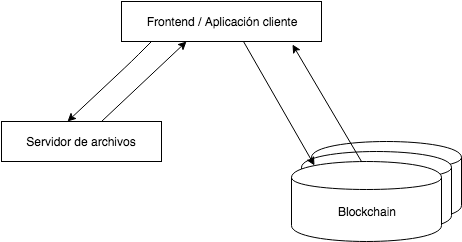
\includegraphics[height=6cm, width=12cm]{arq_sistema.png}
  \centering
  \caption{Arquitectura del sistema}
  \label{fig:arq-sistema}
\end{figure}

Lo que se intenta describir son los tres componentes básicos, es decir, el \textit{frontend}, el servidor de archivos y el \textit{backend} o blockchain, el cual necesariamente estará distribuido y replicado por su naturaleza intrínseca. Habrá interacciones bidireccionales entre el frontend y el servidor de archivos y entre el primero y la blockchain para las distintas operaciones a especificar. Y como se ha dicho anteriormente, opcionalmente el servidor de archivos podría estar replicado y las aplicaciones clientes también, si en futuro, por ejemplo, fueran aplicaciones móviles.

\subsubsection{Control propio de las transacciones}
\label{control_propio_transacciones}

Ahora bien, a partir de aquí se podrían elaborar muchas variantes. Una de ellas, que se ha discutido en un principio, es si introducir en la arquitectura presentada un \textit{backend} propio con control total del proveedor del servicio. Este nuevo planteo brinda algunos beneficios producto de colocar un punto en el medio del canal de comunicación entre los clientes y la blockchain:

\begin{enumerate}
  \item La cuenta para realizar las transacciones hacia la blockchain de Ethereum podría quedar a cargo del proveedor y no de los usuarios, lo cual podría hacer más cómodo y atractivo el servicio para estos últimos. Desde la perspectiva del proveedor, se puede recurrir a la instalación de uno o más nodos dedicados a minar (validar transacciones, muy similar a como se vio en \ref{bc_bitcoin_net_overview}) que ayuden a compensar el gasto transaccional generado por los usuarios.
  \item Podrían facilitarse cuestiones de autenticación y validación de usuarios de una manera más tradicional, y por ende, sencilla de implementar.
\end{enumerate}

A continuación se expondrá un gráfico ilustrativo de esta variante, similar al expuesto en la figura \ref{fig:arq-sistema}:

\begin{figure}[H]
  \includegraphics[height=7cm, width=12cm]{arq_sistema_conbackcentral.png}
  \centering
  \caption{Arquitectura del sistema con backend propio central}
  \label{fig:arq-sistema-conbackcentral}
\end{figure}

La principal desventaja de este modelo es que se deja expuesto un punto de centralización sobre un sistema distribuido, con lo cual, se vuelven a sumar problemas relacionados a la disponibilidad del servicio y a la confianza que, justamente, en una solución sobre la cual se justifica el uso de una blockchain se pretenden evitar. Con lo cual, por esta razón, se decidió trabajar con un modelo totalmente distribuido, es decir, con el frontend comunicándose directamente contra cualquier nodo de la blockchain, de manera tal que si uno de ellos cae, siempre se podrá acceder a otro que esté en funcionamiento y, por otro lado, con la ventaja de poder auditarse públicamente la información alojada en la misma y con la garantía de que la misma nunca fue, es y será alterada (ver \ref{bc_bitcoin_security})

\subsubsection{Resumen de la arquitectura propuesta}
\label{Resumen de la arquitectura propuesta}

Recapitulando lo expuesto en toda esta parte, el diseño de la aplicación consistirá de:

\begin{itemize}
  \item Frontend: una aplicación que brinde las operaciones necesarias al usuario como para listar, verificar y dar de alta certificaciones de archivos.
  \item Servidor de archivos: lugar donde residirán los archivos. Debería proveer por archivo una huella y una identificación unívoca y anónima.
  \item blockchain (Backend): el corazón de la aplicación, en donde se persistirán y distribuirán las huellas de los archivos.
\end{itemize}

\subsection{Especificación de las operaciones}

A continuación se describirán las principales operaciones que permitirá realizar la aplicación. Como se ha dejado establecido, se deberán proveer por lo menos dos casos de uso:

\begin{enumerate}
  \item  La posibilidad de dar de alta certificaciones de archivos
  \item  La posibilidad de listar y verificar las certificaciones de los archivos
\end{enumerate}

\subsubsection{Alta de certificación}
\label{alta_certificacion}

A continuación, se mostrará el diagrama de secuencia pertinente a la operación de alta de una certificación junto con una breve explicación paso a paso:

\begin{figure}[H]
  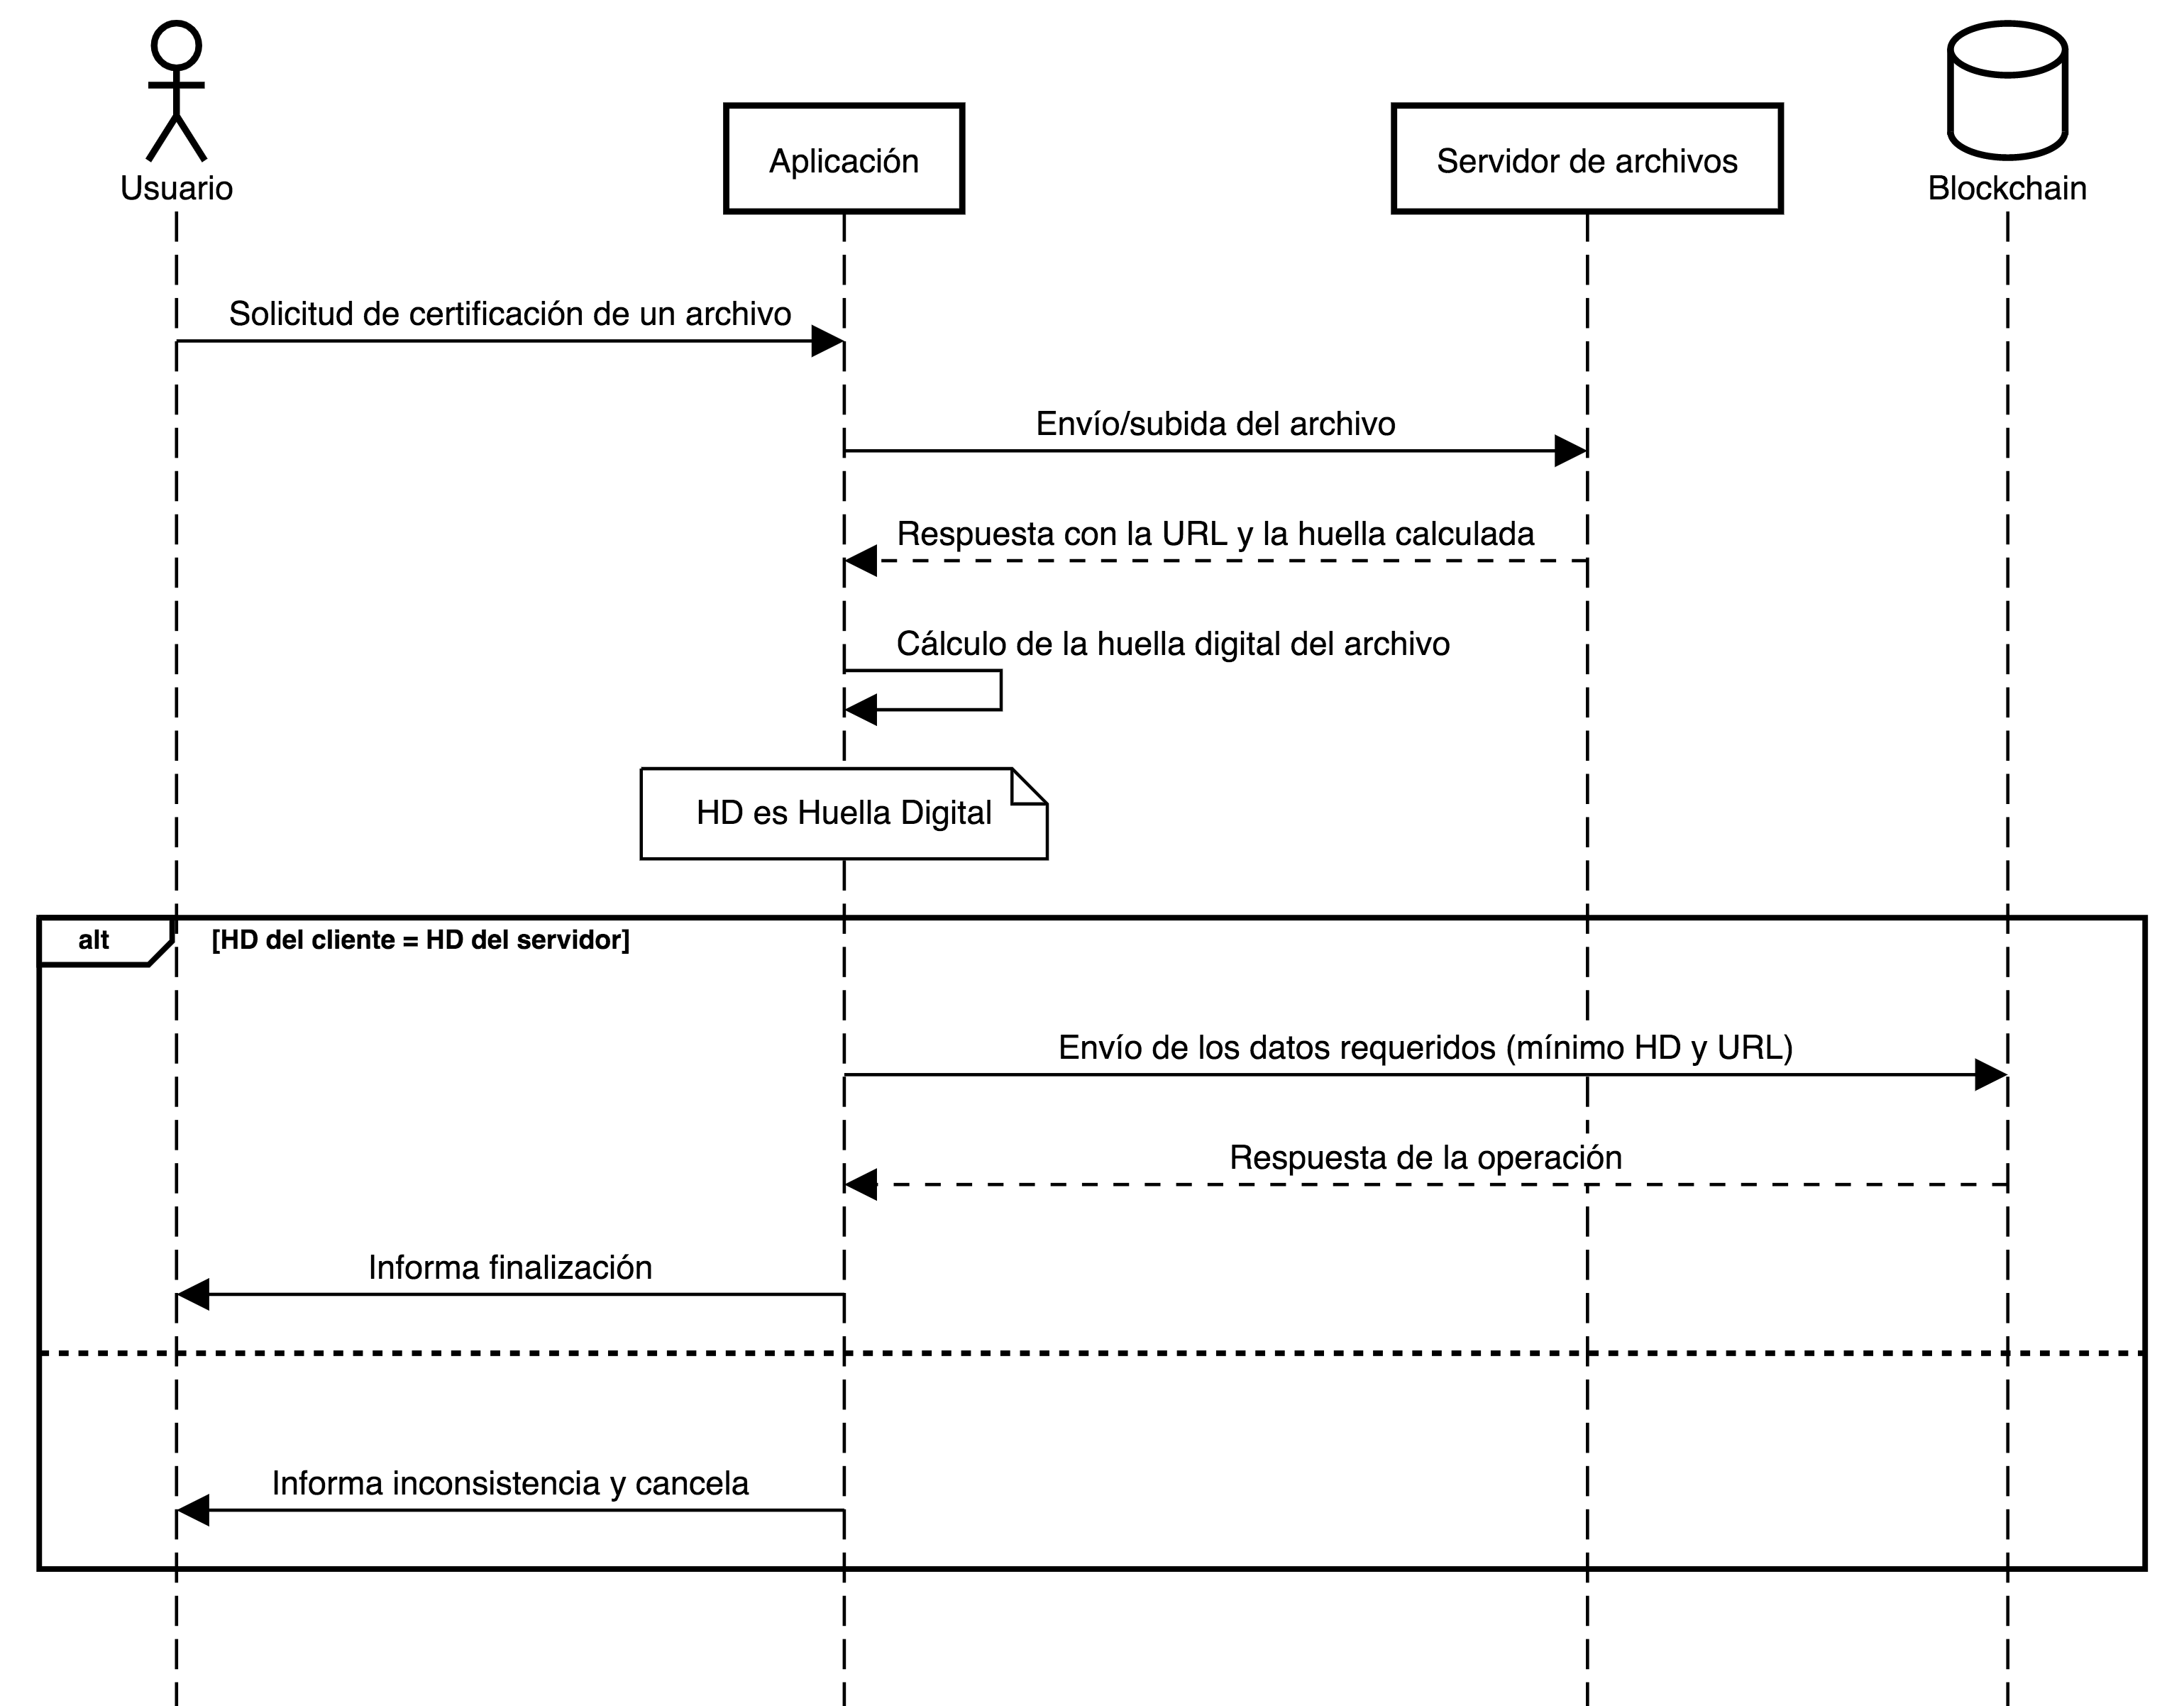
\includegraphics[height=12cm, width=14cm]{upload_certificado_diagrama_secuencia.png}
  \centering
  \caption{Operación alta de certificación}
  \label{fig:upload-certificacion-diagrama-secuencia}
\end{figure}

El primer paso, lógicamente, es solicitar desde el \textit{Frontend} el archivo a certificar. Esto es lo mínimo indispensable como para que esta operación funcione correctamente. Adicionalmente es posible solicitar más información, lo cual se analizará en el apartado \ref{datos_guardar_blockchain}.

El archivo se transfiere hacia el servidor de archivos donde será alojado para futuras consultas y/o descargas. Si esta operación es exitosa, la respuesta que recibirá el \textit{Frontend} será la URL del recurso almacenado y la huella digital del mismo calculada en aquel servidor.

Luego se calcula la huella digital del archivo que ya se encuentra residente en la aplicación \textit{Frontend} y se compara dicha huella con aquella que fue recibida desde el servidor. Si ambas coinciden, se procede con la operación; de lo contrario, se cancela y se informa al usuario. La razón de hacer esta comprobación es para suministrarle al circuito una capa de seguridad adicional en el tramo de transferencia del archivo desde el \textit{Frontend} hacia el servidor de archivos, es decir, si por alguna razón alguien o algo ya sea de manera intencionada o fortuita interfiere en dicho canal de comunicación hacia un componente centralizado (recordar que el servidor de archivos puede ser único), entonces esta verificación servirá para detectar inconsistencias o anomalías en este paso.

Si en este punto todo se encuentra en orden, entonces ahora sí, se procede a la transferencia de la información hacia la blockchain. Nuevamente, lo mínimo que se debería transferir es la huella digital y el identificador del archivo. Opcionalmente se podría empaquetar en dicha transacción otros metadatos útiles para la posterior identificación de la operación de certificación. Cabe destacar que, generalmente, esta funcionalidad puede demorar bastante más que el resto dadas las características inherentes de la blockchain tales como la espera de confirmaciones de algunos nodos y ejecución del contrato inteligente (ver \ref{bc_bitcoin_net_overview} y \ref{bc_ethereum_gas})

Finalmente, si el guardado en la blockchain fue exitoso, se informa al usuario que la operación fue realizada correctamente, y con esto, concluye la operación de certificación.

\subsubsection{Datos a almacenar en la blockchain}
\label{datos_guardar_blockchain}

La idea en esta sección es analizar sucintamente qué datos podrían insertarse dentro de la blockchain, más allá de la indispensable huella digital.

Pero antes, se podría evaluar si, además o en lugar de la huella digital, se podría almacenar el archivo entero dentro de ella. Para los propósitos de este trabajo, dicha opción no resulta conveniente por las siguientes desventajas técnicas y de seguridad que subyacen:

\begin{enumerate}
  \item Subir un archivo a la blockchain podría, en general, exceder los límites de una transacción simple y, además, en el caso particular de la blockchain de Ethereum, también entra en juego la variable del \textit{gas} que tiene un límite máximo por transacción y por bloque (ver \ref{bc_ethereum_gas}); aun ignorando todo esto, sería también potencialmente costoso dado que, justamente, el \textit{gas} insume dinero.
  \item No sería posible subir archivos a una blockchain pública con información sensible. Respecto a esto, cabe destacar que siempre se evitará mostrar información o contenido respecto al archivo. Una vez más, el objetivo es únicamente demostrar que el archivo, a partir de un determinado momento, tiene cierto contenido identificado a través de un sello/huella y, por ende, no podrá cambiar.
\end{enumerate}

Entonces, además de la huella digital, ¿qué otros datos podrían considerarse guardar?

En primer lugar se podría pensar, tal vez, en incluir como dato esencial el momento en el cual se registra la certificación en la blockchain, es decir, una fecha/hora o \textit{timestap} de la operación. Esta afirmación no sólo es válida sino que también es insoslayable: la certificación, justamente, garantiza inmutabilidad del recurso certificado desde un momento determinado, con lo cual, este dato debería ser obligatorio para que esta operación tenga sentido. No obstante, las transacciones -más precisamente los bloques- que se realizan en cualquier arquitectura de tipo blockchain -y en particular, en Ethereum- registran siempre el momento en el cual son creadas, con lo cual, implícitamente esta información siempre está disponible (ver \ref{bc_bitcoin_components} y \ref{bc_ethereum_data_layer}). Como contraargumento se podría mencionar que este dato, devenido de la creación del bloque y la transacción contenida en él, no es exacto puesto a la demora que transcurre entre el momento en el cual se solicita el registro de la certificación en el \textit{Frontend} y el momento en donde efectivamente se confirma la transacción en la red de blockchain. En caso de ser sumamente necesario contar con dicha exactitud se podría registrar aquel momento como dato adicional, solicitándolo desde algún servicio externo que brinde certificación de tiempo en los primeros pasos de la certificación, es decir, antes de transferir el archivo al servidor de archivos.
En segundo lugar podrían enviarse datos referentes al usuario del sistema y/o propietario del archivo a certificar, con el propósito de informar, justamente, quién solicitó dicha operación.
Adicionalmente, otro dato que podría ser útil en algunos contextos es la geolocalización, ya sea registrando las coordenadas o mediante dirección IP. Esto permitiría saber dónde se solicitó la certificación.
Y por último, se podría incluso pensar en dejar un campo libre donde el usuario puede comentar o registrar cualquier información pertinente al proceso de certificación para que quede registrado en la blockchain de forma permanente.

\subsubsection{Listado de certificaciones}
\label{listado_certificaciones}

La operación que lista las certificaciones realizadas en el sistema se describe gráficamente de la siguiente manera:

\begin{figure}[H]
  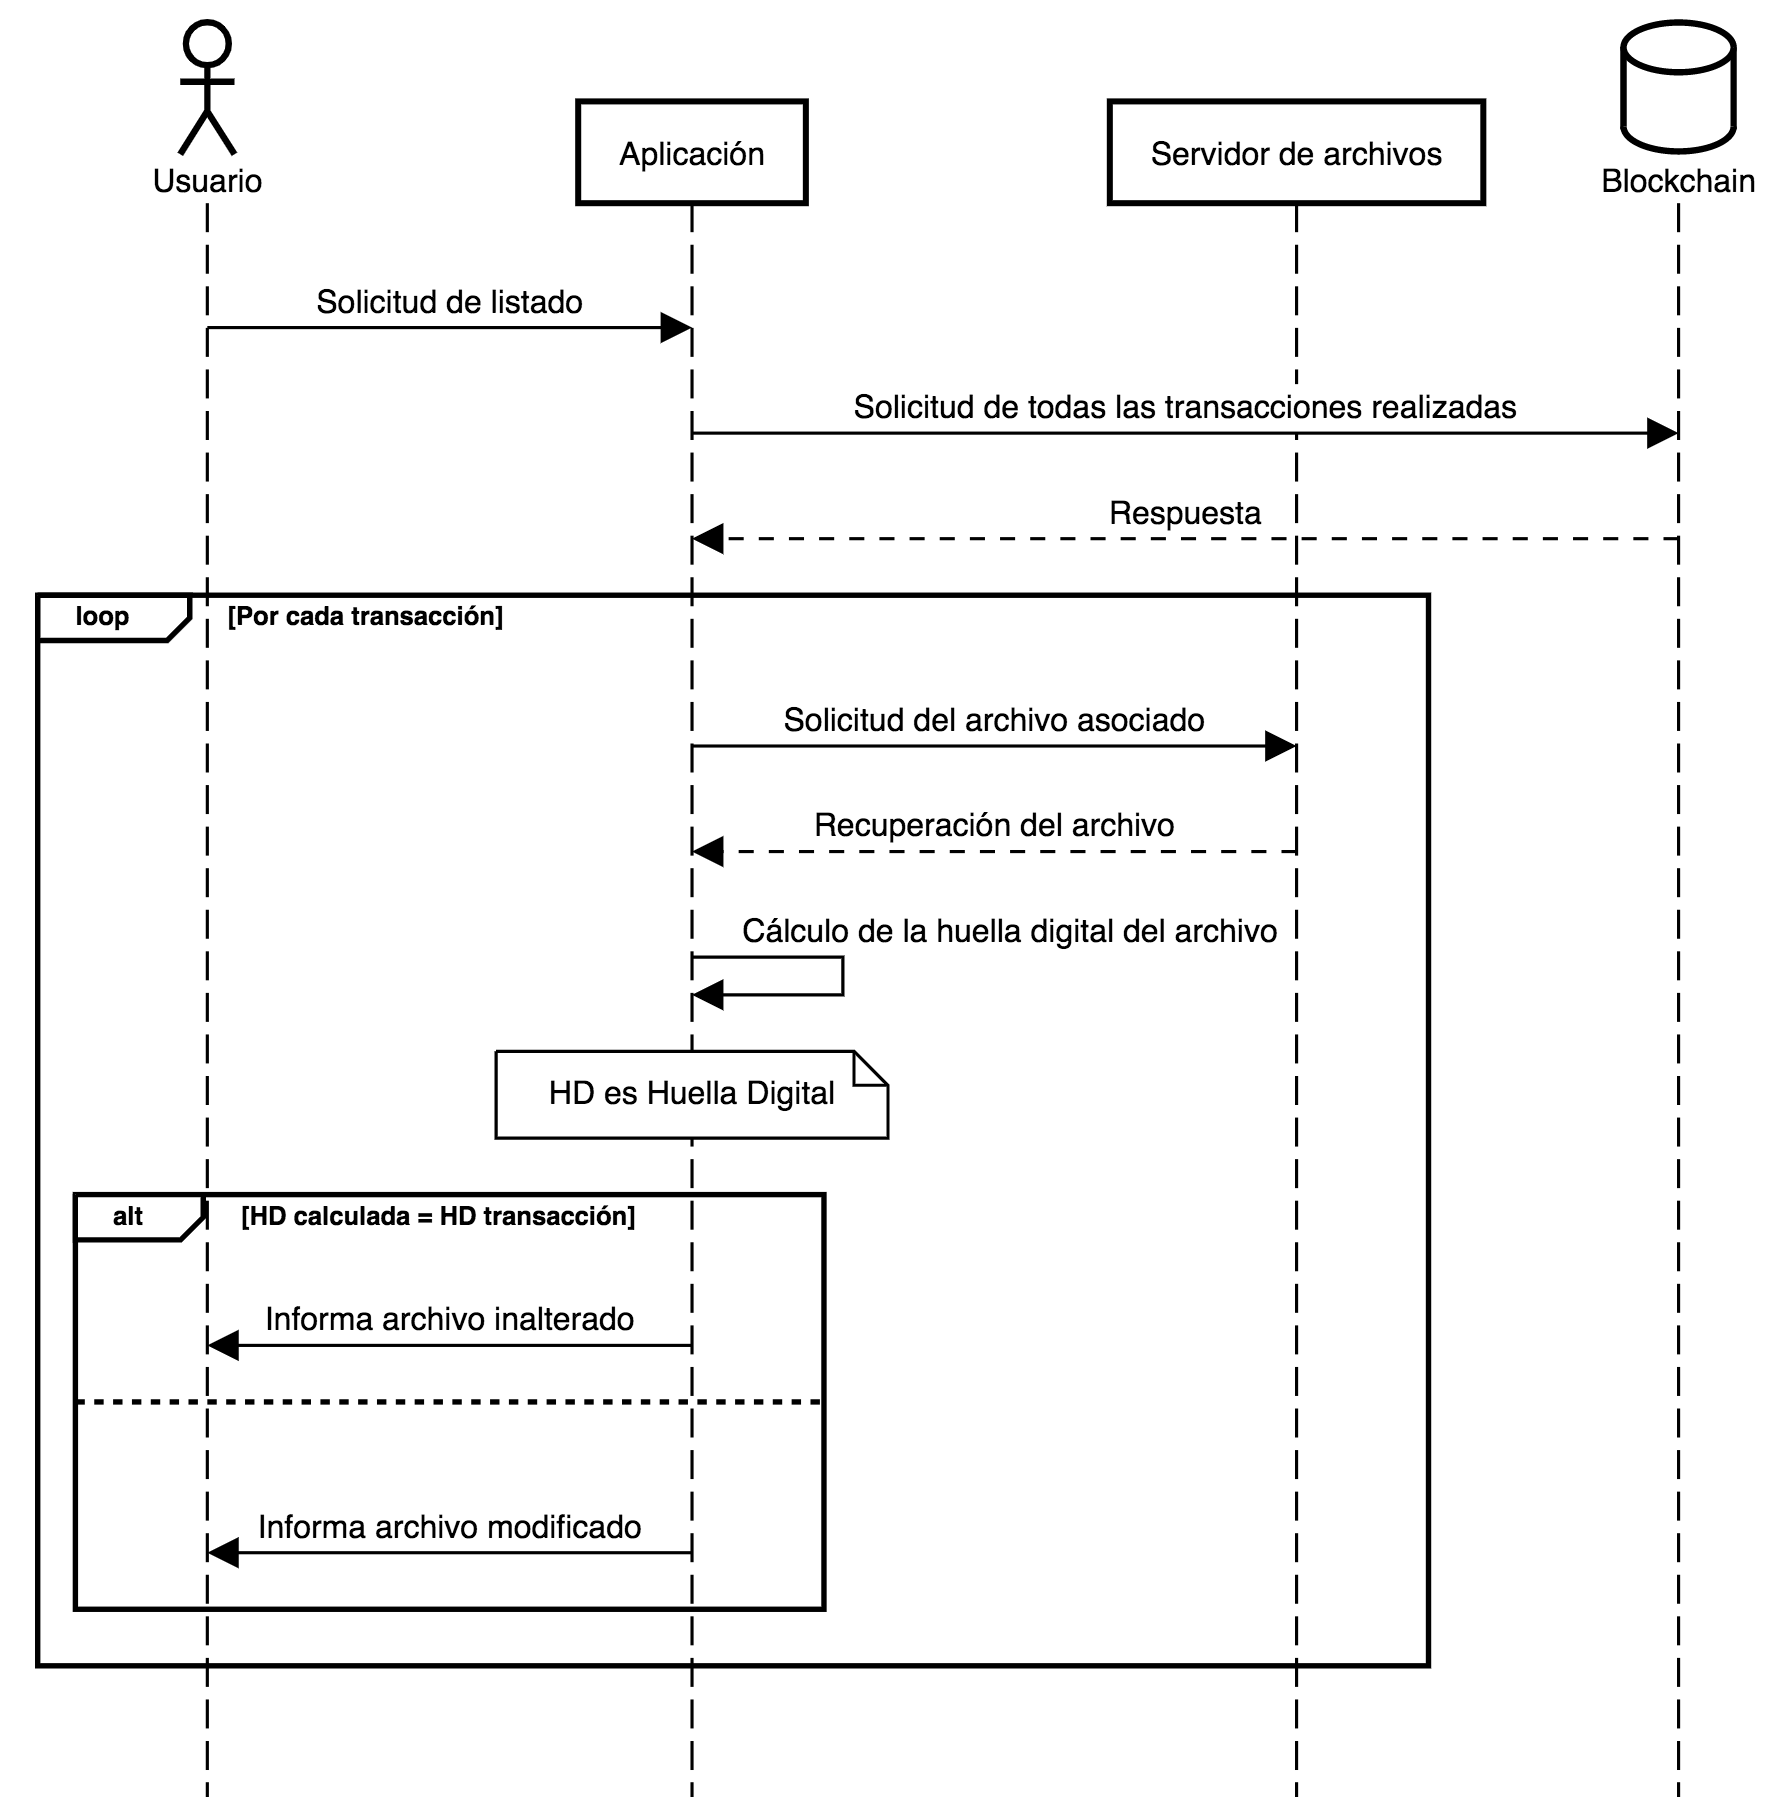
\includegraphics[height=14cm, width=14cm]{listado_certificaciones_diagrama_secuencia.png}
  \centering
  \caption{Operación listado de certificaciones}
  \label{fig:listado-certificaciones-diagrama-secuencia}
\end{figure}

Lo primero que transcurre en esta operación es la solicitud de los datos procedentes de las transacciones que se hicieron sobre la blockchain. Una vez que se recuperan dichas transacciones se procede a obtener, para cada una de ellas, la información del archivo tal como está en ese momento desde el servidor de archivos, a través del identificador que fue registrado durante la certificación, en conjunto con la huella digital.  Una vez realizado esto, se calcula la huella digital de cada uno en el \textit{frontend}, o dicho de manera equivalente, localmente, y se la compara contra la huella digital alojada en la transacción obtenida: si son iguales, significa que no hubo alteraciones desde aquel momento; de lo contrario, entonces el archivo, por alguna razón -ya sea por imperfecciones en la red, en el almacenado del archivo o mediante terceros de manera intencionada o involuntaria-, se vio adulterado.
Toda esta información es mostrada al usuario para que así pueda informarse acerca del estado de integridad de cada uno de los archivos certificados.

\subsection{Implementación de las operaciones}

En esta sección se dará un pantallazo general respecto a la implementación del sistema especificado previamente. Se arrancará primero con el \textit{backend} que estaría representado por el contrato inteligente desplegado en la blockchain de Ethereum, y posteriormente, se verán las implementaciones de las diferentes operaciones que pueden realizarse desde el \textit{frontend}.

\subsubsection{Contrato inteligente (\textit{backend})}

Como se explicó en los capítulos \ref{bc_ethereum_smart_contracts} y \ref{bc_ethereum_evm}, los contratos inteligentes son fragmentos de código que son interpretados y ejecutados por las máquinas virtuales que residen en los nodos mineros de la red, en este caso, Ethereum. Estos están compuestos por un estado -representado mediante variables globales- y funciones que contiene lógica programable que permiten la manipulación de dicho estado -lectura y escritura-. Para programar los contratos inteligentes se pude utilizar distintos tipos de lenguajes, para este caso se decidió utilizar \textit{Solidity}\cite{Solidity2019}. La elección fue tomada teniendo en consideración los siguientes puntos:

\begin{itemize}
  \item Solidity fue diseñado específicamente para la plataforma Ethereum.
  \item La mayor parte de los componentes y librerías que circulan en la red están realizados en Solidity.
  \item Existe gran cantidad herramientas creadas para la construcción, verificación y prueba de los contrato inteligentes desarrollados sobre Solidity.
  \item Es fácil de aprender y utilizar.
\end{itemize}

Una vez dicho esto, se procede al análisis del código y las estructura del contrato, comenzando con las variables de estado necesarias para almacenar la información que compone a la huella digital y luego las funciones que aportan el comportamiento lógico.

\paragraph{Variables de estado del contrato (\textit{backend})}

Solidity provee diferentes tipos de datos y para representar la huella digital se utilizará el tipo \textit{byte} que es un arreglo de longitud dinámica y almacena bytes. Como la huella digital es un dato hexadecimal de 256 bits se podría alocar en un arreglo con una longitud de 32 bytes. Este tipo de arreglo dinámico es especial debido a que existe la posibilidad de declarar dichos arreglos de longitudes fijas. Una diferencia práctica importante entre los arreglos dinámicos y fijos es que los arreglos de longitud fija se pueden usar en argumentos de función para pasar datos o retornar datos fuera del contrato. El tipo \textit{bytes} de longitud variable también se puede utilizar como argumento de funciones, pero solo para uso interno (dentro del mismo contrato), porque la interfaz llamada ABI no permite -al menos por el momento- tipos de longitud variable como retorno de funciones externas. Por lo tanto se utilizará el tipo de dato \textit{bytes32} para almacenar la huella digital.

\begin{minipage}{\linewidth}
  \begin{lstlisting}[frame=single, language=javascript, captionpos=b, caption=Tipo de dato NotarizedFile, belowskip=1em, aboveskip=2em, label={lst:post_archivo}]
    struct NotarizedFile {
        string name;
        string fileUrl;
        uint256 timestamp;
    }
  \end{lstlisting}
\end{minipage}

La palabra reservada \textit{struct} se utiliza para crear estructuras (tipo producto)  de datos definidos por el usuario; su comportamiento y declaración es similar a cualquier lenguaje de programación. En este caso se utilizará para crear la estructura \textit{NotarizedFile} que contendrá los campos referidos a los metadatos de la huella digital:

\begin{enumerate}
  \item name: El nombre del usuario que realizará la certificación.
  \item fileUrl: La dirección URL del lugar físico donde residirá el archivo.
  \item timestamp: La marca de tiempo, la cual determinará la fecha y hora en la que se publicará el bloque de la transacción.
\end{enumerate}

Como se mencionó anteriormente, los datos que componen esta estructura de datos podría ser mayor, dependiendo de las necesidades de la aplicación.

\begin{minipage}{\linewidth}
  \begin{lstlisting}[frame=single, belowskip=1em, aboveskip=2em,  language=javascript, captionpos=b, caption=Variable de estado notarizedFiles, label={lst:post_archivo}]
    mapping (bytes32 => NotarizedFile) public notarizedFiles;
  \end{lstlisting}
\end{minipage}

Una estructura de datos similar a lo que sería una tabla hash clave-valor, es decir que para cada clave del \textit{mapping} existe un valor asociado. Este tipo de dato permite realizar el enlace de la estructura \textit{NotarizedFile} detallada anteriormente y la huella digital del archivo que se representará como un tipo de dato \textit{byte32}.

\begin{minipage}{\linewidth}
  \begin{lstlisting}[frame=single, belowskip=1em, aboveskip=2em,  language=javascript, captionpos=b, caption=Variable de estado filesByHash, label={lst:post_archivo}]
    bytes32[] public filesByHash;
  \end{lstlisting}
\end{minipage}

Un arreglo de tipo \textit{bytes32} para almacenar las huellas digitales de todos los archivos certificados. Esta variable nos permite consultar el número total de archivos certificados por el sistema para obtener un dato estadístico o bien para iterar sobre los mismos.

\paragraph{Funciones del contrato (\textit{backend})}

Dentro de un contrato pueden existir dos tipos de funciones, las que modifican el estado del mismo -escritura- y las que consultan el estado -lectura-. Las que modifican el estado se ejecutan mediante la creación de transacciones y como se mencionó en el apartado \ref{bc_ethereum_smart_contracts} las transacciones tiene un costo, debido a que las mismas quedan alojadas en la blockchain. El costo de las transacciones depende de la cantidad de parámetros enviados y la cantidad de líneas que posee la función y se paga con la criptomoneda nativa de la blockchain donde se ejecuta, en este caso \textit{ether}. Por otro lado existen las funciones de lectura, las cuales no modifican el estado del contrato, por este motivo es que el costo de estas funciones es cero. A continuación se detallarán cada una de las funciones que componen al contrato inteligente de la tesina:

\begin{minipage}{\linewidth}
  \begin{lstlisting}[frame=single, belowskip=1em, aboveskip=2em,  language=javascript, captionpos=b, caption=Función addFile, label={lst:post_archivo}]
    function addFile(
      bytes32 _notarizedHash,
      string calldata _name,
      string calldata _fileUrl
    ) external returns(bool) {
      require(
        bytes(_name).length != 0, "El nombre es requerida"
      );
      require(
        bytes(_fileUrl).length != 0, "La URL es requerida"
      );
      require(
        _notarizedHash.length != 0, "El hash es requerido"
      );
      require(
        notarizedFiles[_notarizedHash].timestamp == 0,
        "El archivo fue agregado previamente"
      );

      notarizedFiles[_notarizedHash].name = _name;
      notarizedFiles[_notarizedHash].fileUrl = _fileUrl;
      notarizedFiles[_notarizedHash].timestamp = now;
      filesByHash.push(_notarizedHash);

      emit FileAdded(_notarizedHash);
      return true;
    }
  \end{lstlisting}
\end{minipage}

La función \textit{addFile} no se puede ser accedida internamente, sólo externamente. Esto es debido a la palabra reservada \textit{external} en la línea 5 que otorga dicho comportamiento, a estas componentes de declaración de funciones se las llama \textit{modificadores de acceso}. La función permite básicamente dar de alta una nueva certificación con la huella digital y los metadatos correspondientes a la misma. Esto conlleva a un cambio de estado y por lo tanto el usuario debe pagar por dicha ejecución. En un primer paso se puede observar que se verifica mediante el uso de \textit{require} que los datos recibidos por paramentos no sean igual a cero, como es así la longitud de la huella digital. Solidity usa estructuras de control de excepciones para el manejo de errores y así evitar que, por ejemplo, el usuario que ejecuta una función de un contrato inteligente no envíe parámetros erróneos. Entonces si la condición dada dentro de \textit{require} es falsa, la transacción es revertida por completo, provocando las siguientes dos consecuencias: el estado del contrato vuelve al mismo valor que poseía antes de ser ejecutada la función y se devuelve al usuario la misma cantidad de \textit{ether} que utilizó para ejecutar dicha función.
Una vez corroborado que los parámetros son válidos se procede al almacenamiento de la información: como se puede ver de la línea 20 a la 22 se almacenan en el \textit{mapping} \textit{notarizedFiles} como valor los metadatos y como clave la huella digital y en la línea 23 se agrega la huella al arreglo de huellas. Por último se emite el evento \textit{FileAdded} y se retorna el valor true para confirmar el éxito de la transacción. Los eventos, en \textit{Solidity}, son la forma de alertar a las aplicaciones descentralizadas que se produjo un cambio en el estado de un contrato.

\begin{minipage}{\linewidth}
  \begin{lstlisting}[frame=single, belowskip=1em, aboveskip=2em,  language=javascript, captionpos=b, caption=Función removeFile, label={lst:post_archivo}]
    function removeFile(bytes32 _notarizedHash) external {
        require(
            _notarizedHash.length != 0,
            "El hash es requerido"
        );
        require(
            notarizedFiles[_notarizedHash].timestamp != 0,
            "El archivo no existe"
        );

        notarizedFiles[_notarizedHash].name = "";
        notarizedFiles[_notarizedHash].fileUrl = "";
        notarizedFiles[_notarizedHash].timestamp = 0;
        _removeHash(_notarizedHash);

        emit FileRemoved(_notarizedHash);
    }
  \end{lstlisting}
\end{minipage}

La función \textit{removeFile} también sólo puede ser accedida externamente y elimina un registro de una huella digital dentro del contrato. Se sabe que debido a la naturaleza de la blockchain los datos ingresados dentro de la misma son inmutables, por lo tanto esta función tiene como objetivo demostrar que la única forma de borrar información en un contrato es realizando un borrado lógico. Para ello igual que en la función anterior se verifica que los parámetros que recibe la función sean válidos y luego se procede al borrado. El proceso consiste en darle valores por defecto a los campos de los metadatos asociados a la huella que se desea borrar. Como segundo paso se ejecuta la función \textit{\_removeHash} que elimina la huella del arreglo de huellas, su proceso se detallará más adelante. Y como paso final se emite el evento para alertar a las aplicaciones descentralizadas.

\begin{minipage}{\linewidth}
  \begin{lstlisting}[frame=single, belowskip=1em, aboveskip=2em,  language=javascript, captionpos=b, caption=Función \_removeHash, label={lst:post_archivo}]
    function _removeHash(bytes32 _hash) private {
        uint length = filesByHash.length;
        for (uint i = 0; i < length; i++) {
            if (filesByHash[i] == _hash) {
                filesByHash[i] = filesByHash[length-1];
                filesByHash.length--;
                return;
            }
        }
    }
  \end{lstlisting}
\end{minipage}

La función \textit{\_removeHash} posee el modificador de acceso \textit{private} lo cual indica que sólo permite ser ejecutada internamente a través de otra función que pertenezca al contrato donde está declarada. Tiene como fin eliminar una huella digital dentro del arreglo de huellas. Consiste en la búsqueda de la posición de la huella a eliminar y una vez ubicada se procede a reemplazar la huella de esa posición por la de la última posición. Por último se reduce el tamaño del arreglo en uno. Igual que en la función \textit{removeFile} el borrado es lógico y si se quiere obtener los valores de la huella digital eliminada, sólo se tiene que observar cómo está compuesta la transacción que originó dicho registro.

\begin{minipage}{\linewidth}
  \begin{lstlisting}[frame=single, belowskip=1em, aboveskip=2em,  language=javascript, captionpos=b, caption=Función getFileByHash, label={lst:post_archivo}]
    function getFileByHash(bytes32 _notarizedHash)
        external
        view
        returns(string memory, string memory, uint256)
    {
        require(_notarizedHash.length != 0, "El hash es requerido");
        require(notarizedFiles[_notarizedHash].timestamp != 0, "El archivo no existe");

        NotarizedFile memory notarizedFile = notarizedFiles[_notarizedHash];
        return (
            notarizedFile.name,
            notarizedFile.fileUrl,
            notarizedFile.timestamp
        );
    }
  \end{lstlisting}
\end{minipage}

En la función \textit{getFileByHash} se puede observar en la línea 3 que se presenta la palabra reservada \textit{view} en la declaración de la misma. Esto indica que esta función no va a realizar cambios de estado, solo operaciones de lectura. Esta función permite obtener los metadatos de una huella digital pasada como parámetro: primero realiza las verificaciones sobre el parámetro de entrada y luego retorna los metadatos correspondientes. El valor de esta ejecución es 0 y no se realiza una transacción para obtener los datos.

\begin{minipage}{\linewidth}
  \begin{lstlisting}[frame=single, belowskip=1em, aboveskip=2em,  language=javascript, captionpos=b, caption=Función getNumberOfFiles, label={lst:post_archivo}]
    function getNumberOfFiles() external view
        returns(uint256)
    {
        return filesByHash.length;
    }
  \end{lstlisting}
\end{minipage}

La función \textit{getNumberOfFiles} retorna la cantidad de huellas certificadas hasta el momento de la ejecución. Es una función externa y no realiza modificaciones en el estado del contrato.

En conclusión, teniendo en cuenta que los contratos una vez desplegados en la blockchain no se pueden modificar, se tuvo en cuenta ciertas prácticas que agilizan el proceso de codificación y aportan seguridad al mismo, tales como:

\begin{itemize}
  \item Mantener el código del contrato simple debido a que la complejidad aumenta la probabilidad de errores.
  \item Asegurar que la lógica del contrato sea simple.
  \item Verificar que los parámetros recibidos sean válidos y luego actualizar el estado.
  \item Utilizar la blockchain solo para las partes del sistema que requieran descentralización.
\end{itemize}

\subsubsection{Detalles del servidor de archivos}
\label{detalles_servidor_archivos}

El servidor de archivos se ha desarrollado en Node (Javascript) usando una librería llamada Express.js, la cual provee lo justo y necesario para implementar fácilmente una aplicación web, definiendo puntos de acceso HTTP (\textit{endpoints})\cite{ExpressJS2018}.
En el presente trabajo, lo que se ha hecho fue implementar un único punto de acceso con el propósito de recibir y alojar en el sistema de archivos, el archivo a certificar en la operación de alta. Recordar de \ref{alta_certificacion} que se ha mencionado que el \textit{frontend} requiere desde el servidor de archivos la URL del archivo y la huella digital calculada en él. Por ende, esta información es la que se enviará como parte de la respuesta HTTP del servidor ante la petición de almacenado del archivo sobre el mencionado punto de acceso.
A continuación se mostrará el código del punto de acceso:

\begin{minipage}{\linewidth}
\begin{lstlisting}[frame=single, belowskip=1em, aboveskip=2em,  language=javascript, captionpos=b, caption=Punto de acceso para almacenar archivo, label={lst:post_archivo}]
  router.post('/uploads', function(req, res, next) {
    let uploadedFile = req.files.file;

    uploadedFile.mv(
      `${__dirname}/../public/uploads/${uploadedFile.name}`,
      (err) => {
        if (err) {
          return res.status(422).send(err);
        }

        const digest = sha256(uploadedFile.data)
        res.json({
          file: `uploads/${uploadedFile.name}`,
          digest: digest
        });
    });
  });
\end{lstlisting}
\end{minipage}

Sin entrar en grandes detalles, la intención de la extracto precedente es definir una ruta en la aplicación web, más precisamente un HTTP POST a \textit{/uploads}. En el cuerpo de la petición se requerirá recibir un archivo -el archivo a certificar- (línea 2) y luego se procederá a mover dicho archivo a una carpeta específica dentro del servidor (línea 4-5). Si este procedimiento fallase -ya sea porque no existe el archivo o porque hubo un problema interno en el servidor- , entonces se enviará una respuesta HTTP 422 (entidad sin procesar) con el error. Si no, en la línea 11 se hará el cálculo de la huella digital del archivo y se responderá con el dato de esta huella junto a la URL o identificador del archivo (línea 12-15).
Para los objetivos de esta tesina, este sencillo punto de acceso es suficiente para mostrar un prototipo básico de servidor de archivos.

\subsubsection{Detalles del \textit{frontend}}

Antes de mostrar en detalle las operaciones del \textit{frontend} será conveniente mencionar algunas características y decisiones previas sobre el desarrollo del mismo.
La base de código de la aplicación fue desarrollada en React, una librería hecha en lenguaje Javascript específicamente diseñada para construir interfaces de usuario de manera declarativa por medio de componentes \cite{React2018}
Para la interacción con el contrato desplegado en la blockchain de Ethereum se empleó una librería llamada Web3, la cual provee la funcionalidad necesaria para comunicarse con un nodo cualquiera dentro de la red de Ethereum \cite{Web32018}.
Por último, se ha hecho uso de un plugin de navegador web denominado Metamask, el cual brinda una \textit{criptobilletera} o \textit{wallet} donde se resguarda la criptodivisa con la cual se realizará el pago de las operaciones dentro de la blockchain. Además, provee el acceso a la red con la cual se harán las operaciones, esto quiere decir, que la red que el usuario elija será la que usará Web3 para conectarse y realizar la interacción con la blockchain y el o los contratos \cite{Metamask2018}. La ventaja de esto es que, además de la red Ethereum original (de producción), también se cuentan con redes de testeo de diferentes grados -algunas tan grandes como la de producción y otras mucho más acotadas-, muy útiles para el desarrollo y la verificación de los contratos y de las aplicaciones que hacen uso de los servicios que estos suministran. Por ejemplo, durante el desarrollo del presente trabajo se ha usado la red de testeo Kovan que, a diferencia de la red productiva de Ethereum, es mucho más pequeña y utiliza un protocolo de consenso \textit{Proof-of-Authority} (ver \ref{bc_ethereum_consensus}), el cual es mucho más rápido que el usado por Ethereum.

\subsubsection{Operación de alta de certificación (\textit{frontend})}
\label{operacion_alta_certificacion}

La operación de alta de una certificación es una de las principales funcionalidades que ofrece el sistema. La idea, tal como se describió en el apartado \ref{alta_certificacion} es solicitar algunos datos necesarios para iniciar el procedimiento que, en particular, para este trabajo dichos datos son: la identidad del propietario del archivo a certificar y el archivo en sí. Tal como se ha discutido en la sección \ref{datos_guardar_blockchain} también se podrían haber tenido en cuenta otros datos (y de hecho hay información implícita que se puede extraer desde la transacción o el bloque, como por ejemplo, la fecha y la hora), pero en principio, los mínimos que se le pueden exigir a un usuario son estos. A continuación se mostrará una captura de pantalla de este formulario:

\begin{figure}[H]
  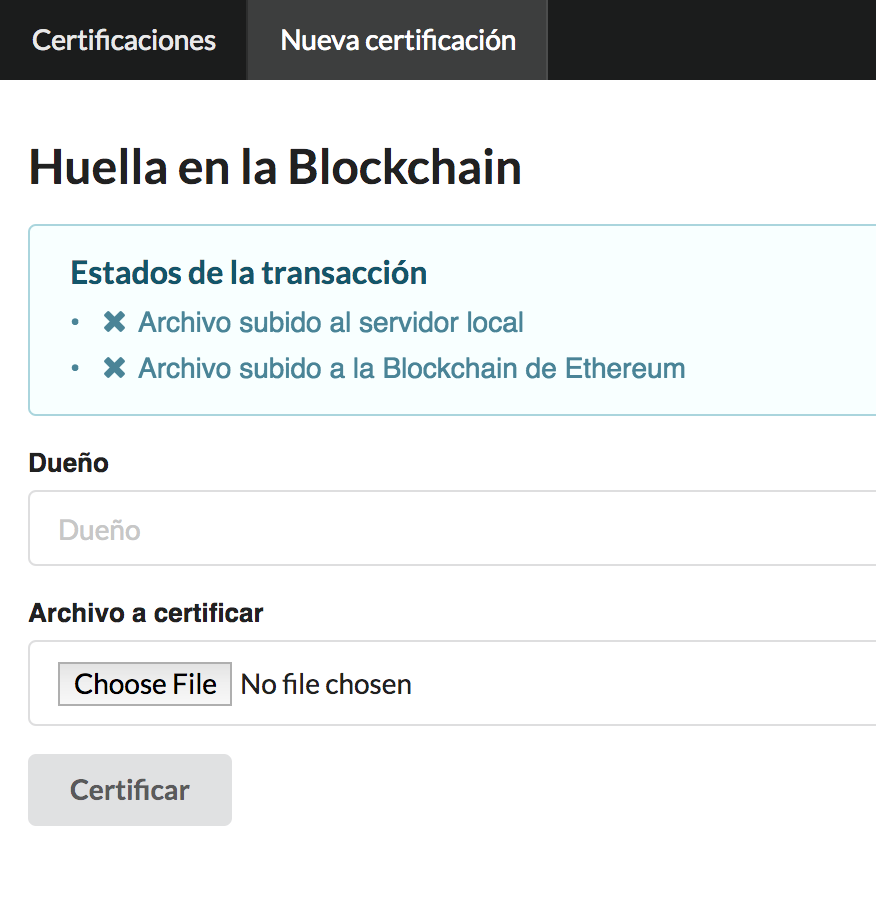
\includegraphics[height=13cm, width=13cm]{alta_certificacion_inicial_sys.png}
  \centering
  \caption{Formulario para dar de alta una certificación}
  \label{fig:alta-certificacion-inicial-sys}
\end{figure}

Aparte de los campos descriptos en el párrafo anterior, se puede ver en la parte superior del formulario un cartel con la leyenda ``Estados de la transacción''. Esencialmente, la transacción dentro del sistema presenta dos estados: el primero en el cual el archivo es transferido al servidor de archivos. A modo de ejemplo, se puede ver en la siguiente imagen:

\begin{figure}[H]
  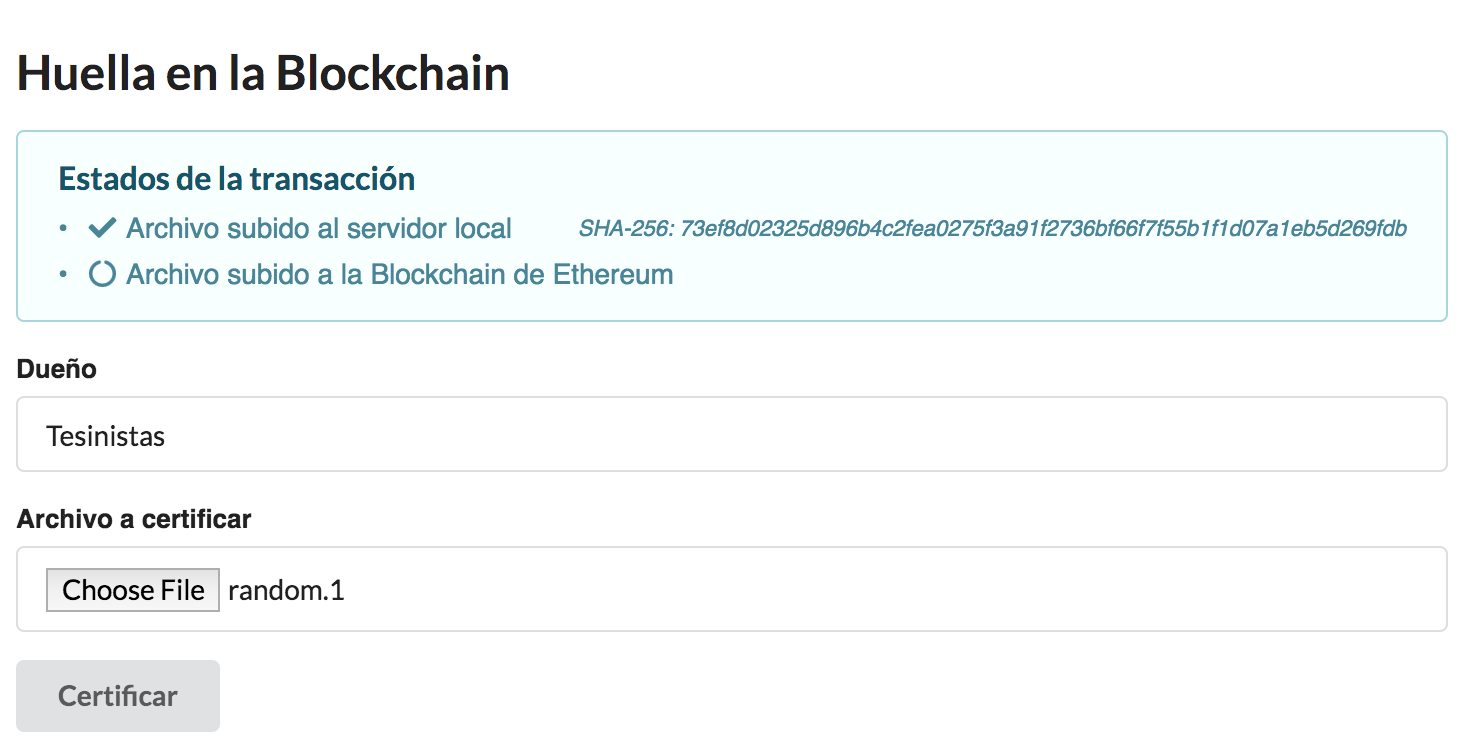
\includegraphics[height=8cm, width=15cm]{alta_certificacion_infs_sys.png}
  \centering
  \caption{Fase 1 completada o transacción en estado 1}
  \label{fig:alta-certificacion-infs-sys}
\end{figure}

Como el propietario ``Tesinistas'' intenta certificar el archivo ``random.1'' y a continuación -tras haber hecho click en el botón ``Certificar''- se puede constatar que las huellas digitales calculadas tanto por el servidor anteriormente nombrado como por la aplicación cliente coinciden, al mismo tiempo que se informa en pantalla. En caso de no coincidir, se informa el problema y se cancela la operación. Con este paso finaliza la fase 1 de la transacción.

Luego, la transacción continua hacia el segundo estado o fase en donde se ejecuta la operación del contrato en la blockchain de Ethereum que tiene como propósito resguardar y difundir el acto certificatorio a través de toda la red. Dado que se necesita hacer uso de una operación de escritura sobre la blockchain de Ethereum (ver \ref{bc_ethereum_smart_contracts}) es necesario realizar el pago correspondiente por el costo de dicha operación, es decir, el costo de ejecutar y registrar en una transacción dentro de dicha red los datos correspondientes a la certificación que se está intentando realizar. Para esta situación, automáticamente se va a desplegar una ventana del plugin \textit{Metamask} para poder autorizar una transferencia de criptomonedas desde la cuenta que solicita la certificación hacia la blockchain. A continuación se mostrará una imagen de ejemplo:

\begin{figure}[H]
  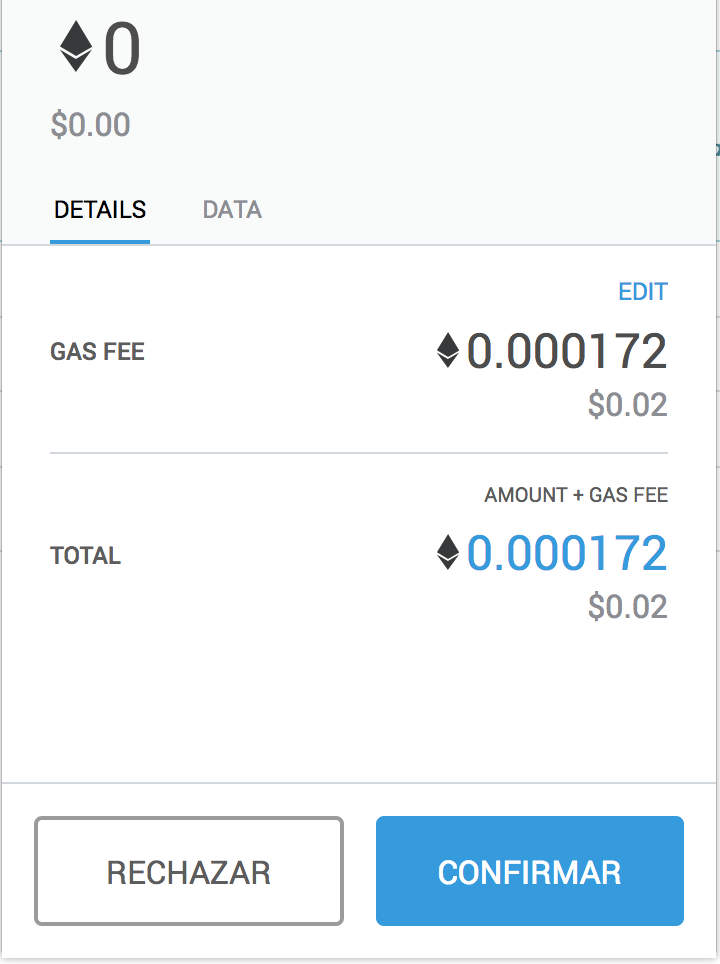
\includegraphics[height=12cm, width=8cm]{alta_certificacion_metamask_sys.png}
  \centering
  \caption{Ventana de Metamask para autorizar la transacción en la blockchain}
  \label{fig:alta-certificacion-metamask-sys}
\end{figure}

Ninguna de las operaciones del contrato implementado para este trabajo cobra un adicional diferenciado por el uso del servicio (recordar \ref{bc_ethereum_smart_contracts}), en cambio, lo que sí se cobra, y es obligatorio siempre, es el \textit{gas} requerido para la realización de la transacción en la blockchain, tal como se explicó en [ref. Gas en Ethereum]. Esta información se puede ver reflejada en imagen expuesta anteriormente es donde se ve, a partir de los datos recabados por Metamask, que el arancel de la operación es 0 mientras que la tasa del \textit{gas} es una fracción de Ether, la moneda usada dentro de Ethereum.

Al confirmar esta transacción, se tendrá que esperar unos momentos -en el orden de algunos minutos- a que la misma se concilie, se difunda y se asiente por varios de los nodos de la red blockchain (muy similar a lo descrito en \ref{bc_bitcoin_net_overview} y \ref{bc_bitcoin_security}) y, finalmente, si todo sucede exitosamente, entonces la operación quedará definitivamente confirmada, a saber:

\begin{figure}[H]
  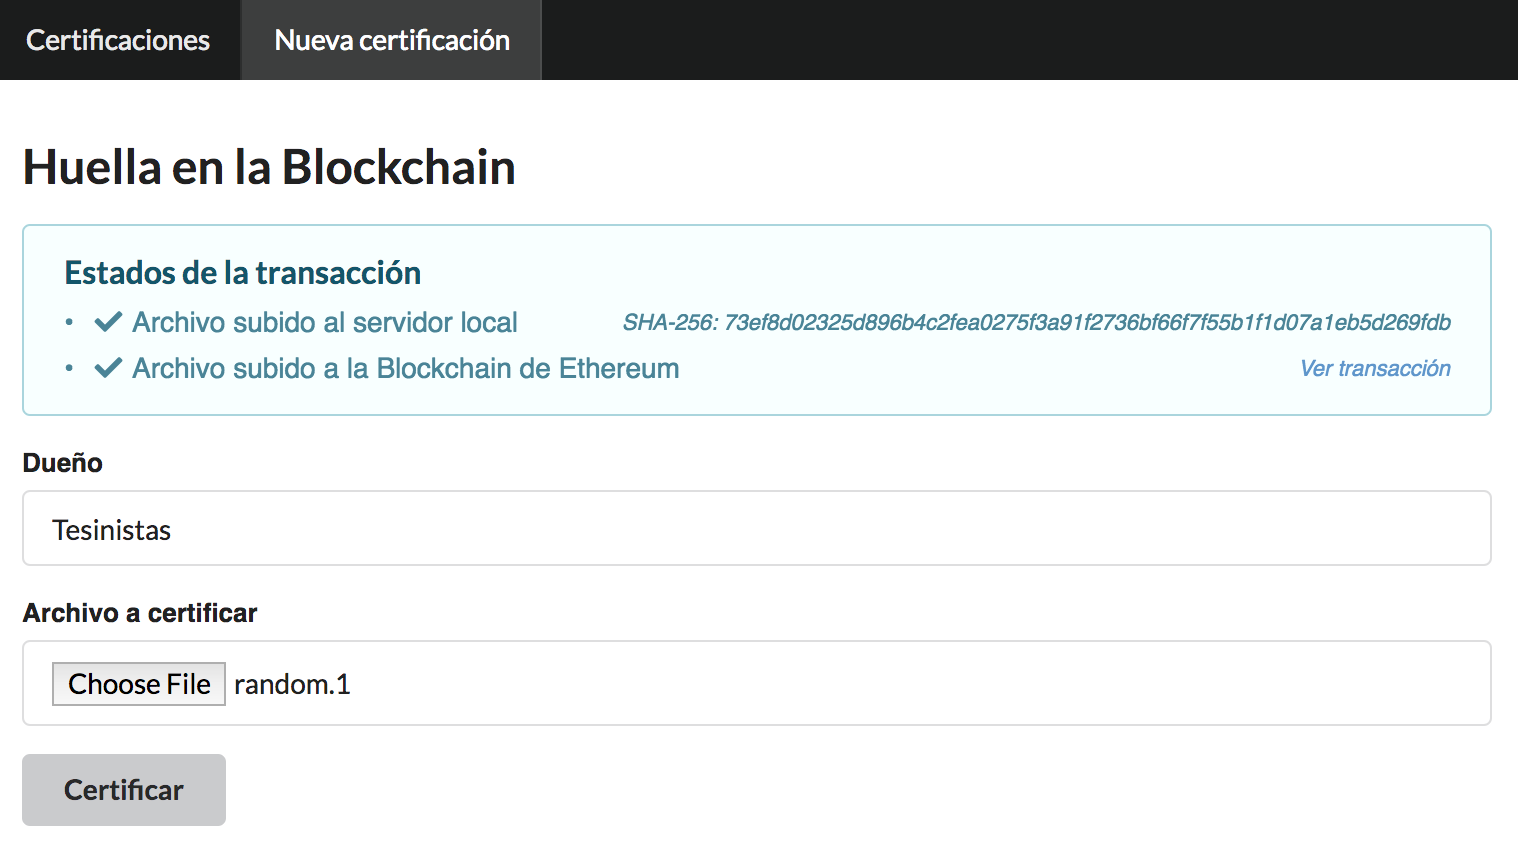
\includegraphics[height=8cm, width=13cm]{alta_certificacion_final_sys.png}
  \centering
  \caption{Transacción registrada en la blockchain y operación completa}
  \label{fig:alta-certificacion-final-sys}
\end{figure}

En la imagen hay un enlace para poder ver el detalle de la transacción registrada por fuera de este sistema, y se explicará con más detalles en la sección \ref{transacciones_blockchain_provider_publico}.

Con el objeto de entender algunos detalles adicionales, a continuación, se introducirá el código que encapsula toda la lógica anteriormente descripta:

\begin{minipage}{\linewidth}
\begin{lstlisting}[frame=single, belowskip=1em, aboveskip=2em,  language=javascript, captionpos=b, caption=Código de alta de certificación, label={lst:alta_certificacion}]
  const file  = this.uploadInput.files[0]
  const owner = this.ownerInput.value
  const data  = new FormData();
  data.append('file', file);
  // Starting upload process to file server
  this.setState({ fileUploadLocalServerStatus: 'pending' })
  calculateDigest(file)
    .then(digestFromClient => {
      axios.post(config.fileserver.endpoint, data)
        .then((response) => {
          const { digest: digestFromServer, file } = response.data
          if (digestFromServer === digestFromClient) {
            this.setState({ digest: digestFromClient, fileUploadLocalServerStatus: 'done' })
            // Listen to blockchain event
            CertContractApi.once('FileAdded', (error, postData) => {
              if (!error) {
                this.setState({ fileUploadEthereumblockchainStatus: 'done', txHash: postData.transactionHash })
              } else {
                console.error('Fallo algo en la subida a la blockchain de Ethereum')
              }
            })
            // Call the contract
            const prefix = '0x' + digestFromClient
            this.setState({ fileUploadEthereumblockchainStatus: 'pending' })
            CertContractApi.addFile(prefix, owner, file)
          } else {
            console.error('Error! Digest cliente != digest servidor')
          }
        })
    })
\end{lstlisting}
\end{minipage}

Lo primero que transcurre, entre las líneas 1-4, es la obtención de los datos del formulario. A partir de la línea 5 comienza a subirse el archivo al servidor de archivos: en 6 se señaliza que esta operación se encuentra pendiente (esto da comienzo a la fase 1 anteriormente descripta). En la línea 7 se procede a calcular la huella digital del archivo dispuesto en el formulario, es decir, en la aplicación cliente, haciendo uso de promesas\footnote{Una promesa es una estructura que permite secuenciar cómputos de naturaleza asincrónica con el objeto de facilitar la lectura del código}. Luego de obtener la huella, se realiza la conexión remota contra el servidor de archivos (linea 9) cuyo funcionamiento fue detallado en \ref{detalles_servidor_archivos}. Si todo transcurre exitosamente, entonces, como se puede ver en la línea 11, se recibirá como respuesta la huella digital calculada por el servidor y la URL del archivo. En 12 se comparan ambas huellas: si no son iguales, se informa el error y se cancela la operación; en caso de ser iguales, se señaliza el fin de la subida del archivo -fase 1- en la línea 13.
En la línea 15 se registra un manejador para un evento. Esto es una práctica común en Javascript y en Node.JS dado que buena parte del desarrollo en estas tecnologías están orientadas a eventos y procesamiento que ocurre asincrónicamente y, consecuentemente, esto favorece el rendimiento (ver, por ejemplo, \cite{TilkovVinoski2010}). En este caso particular, es prácticamente menester usar un mecanismo asincrónico porque la interacción con la blockchain es relativamente muy lenta, y así se evita retrasar el resto de las funcionalidades de la aplicación. El evento particular, para este código que se está describiendo, es \textit{FileAdded}, el cual se dispara cuando la transacción en la blockchain se completa, ya sea exitosamente o con errores. Sea cual sea el caso, cuando el evento se genera, se ejecuta la función asociada a él en donde se puede ver, en la línea 17, que se vuelve a hacer uso de la señalización para cambiar el estado de la operación -marcando el fin de la fase 2- y, con esto, dar fin a la operación.
Luego de registrar el evento, el último paso es realizar el llamado asincrónico a la operación de agregar el archivo en la blockchain (línea 25). Cabe destacar que tanto aquí, como en el registro del evento, se hace uso de un módulo llamado \textit{CertContractApi} el cual abstrae y separa toda la interacción contra la blockchain mediante la librería Web3 (de hecho, en ninguna de las operaciones se ve su uso por si en un futuro se decide cambiar la librería que provee las facilidades para comunicarse con la blockchain de Ethereum)

\subsubsection{Operación de listar certificaciones (\textit{frontend})}

Otra de las grandes funcionalidades que ofrece el sistema es la posibilidad de ver el listado de las transacciones ejecutadas junto a una verificación sobre el estado de inmutabilidad de los archivos asociados. En la sección \ref{listado_certificaciones} ya se repasó a alto nivel el flujo y las interacciones que intervienen en este requerimiento. A partir de ahora, se hará una explicación más detallada mostrando código e imágenes de esta operación

\begin{figure}[H]
  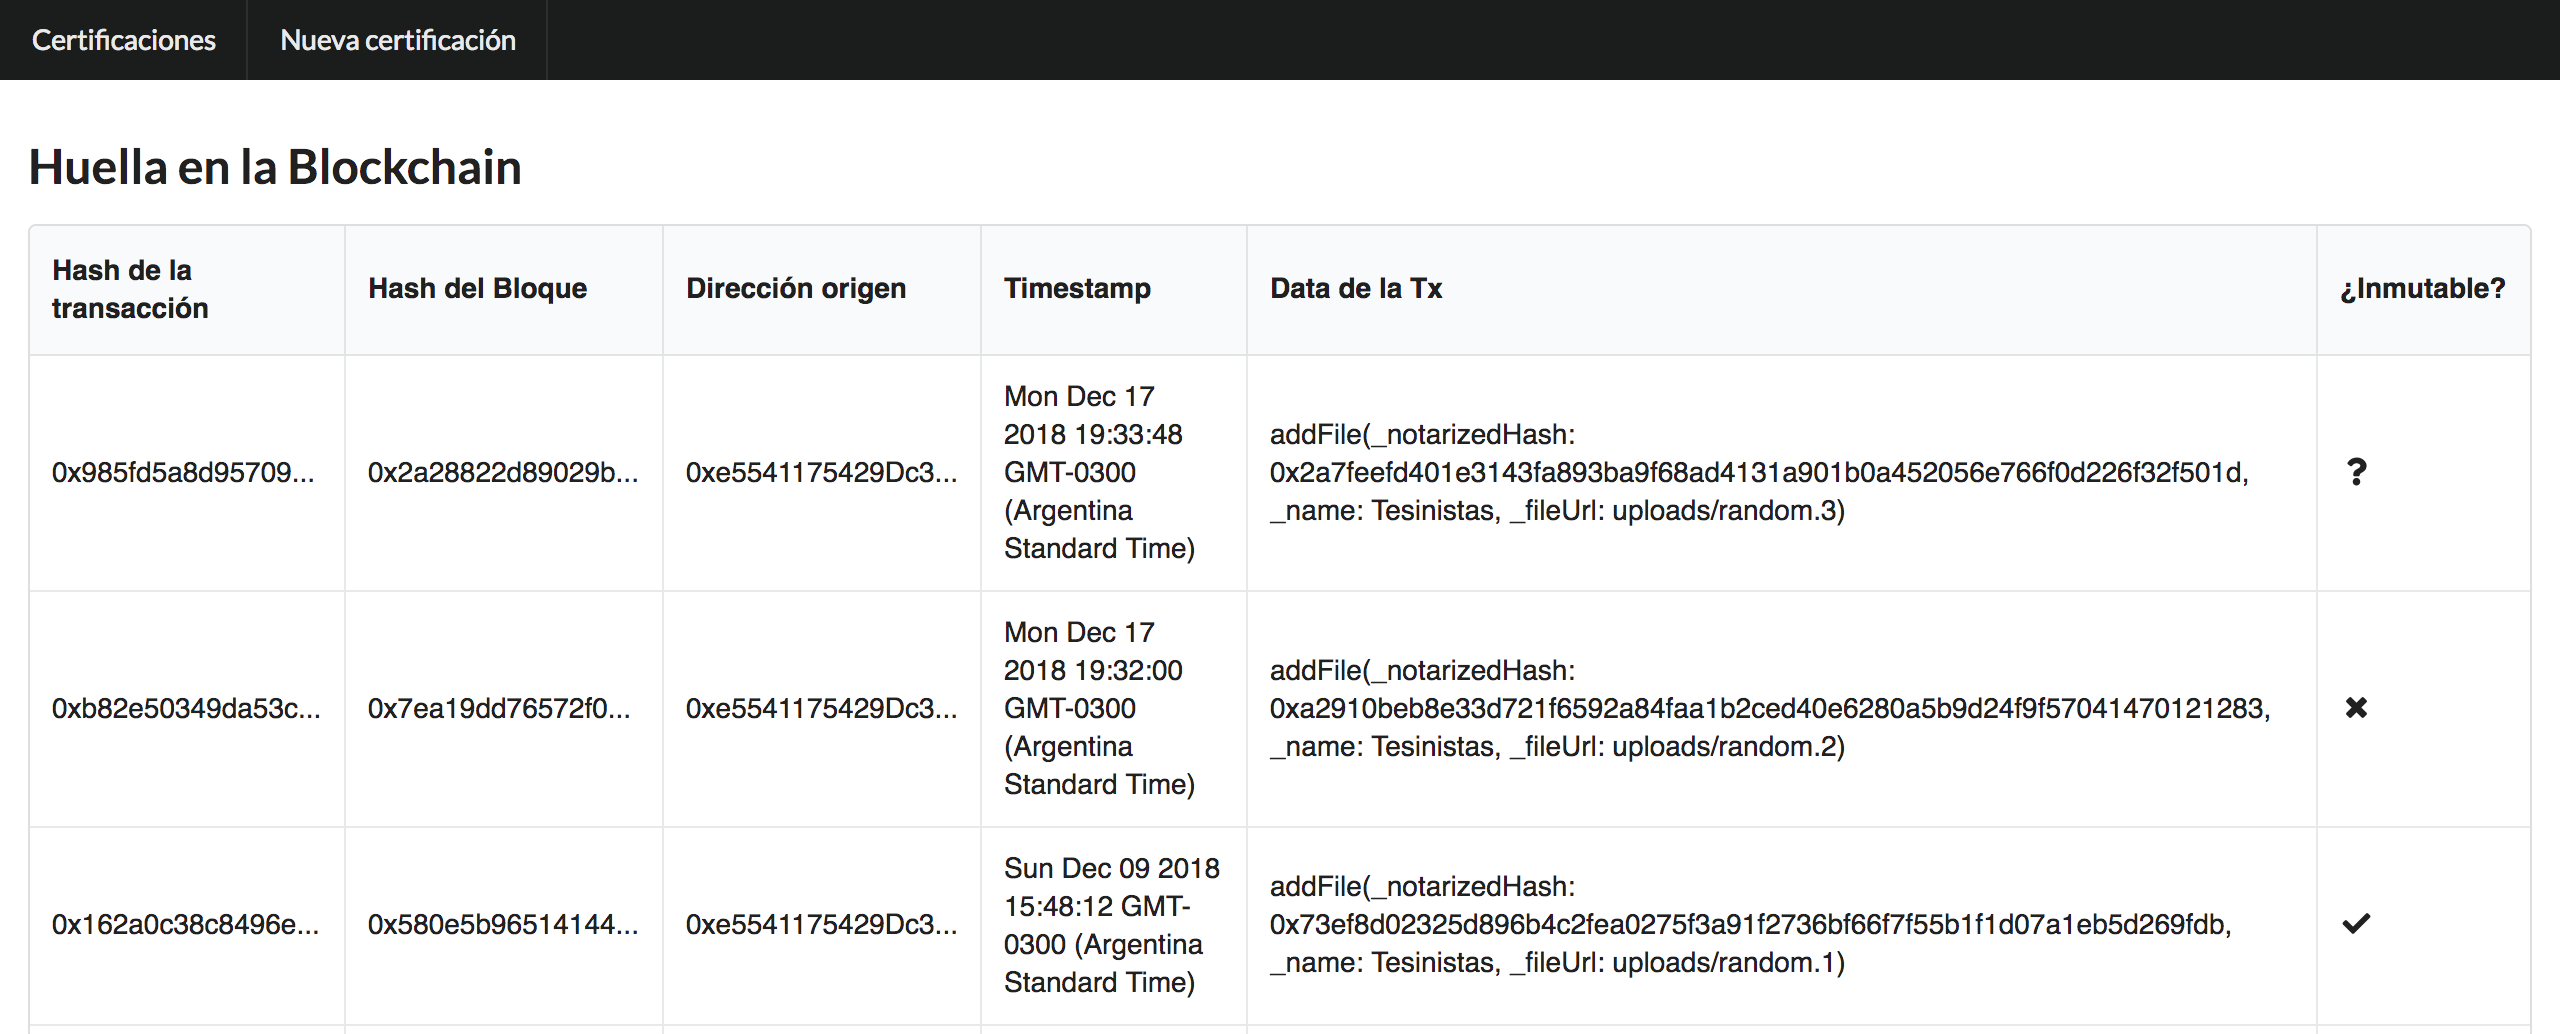
\includegraphics[height=6cm, width=13cm]{listado_certificaciones_ej.png}
  \centering
  \caption{Ejemplo de listado de certificaciones}
  \label{fig:listado-certificaciones}
\end{figure}

Como se puede ver en la imagen anterior, lo que se muestra son las últimas tres transacciones realizadas en el sistema. Cabe destacar en este punto que las transacciones listadas en esta vista provienen directamente de la blockchain, con lo cual, todos los datos -excepto los ``datos propios''- son extraídos exclusivamente de los metadatos de las transacciones guardadas en dicha base de datos. De cada una se puede ver la siguiente información:

\begin{itemize}
  \item \textbf{Hash de la transacción:} constituye la huella digital de una transacción. Permite identificarla unívocamente entre todas las transacciones almacenadas en la blockchain.
  \item \textbf{Hash del bloque:} constituye la huella digital de un bloque, el cual, como ya se ha explicado en \ref{bc_bitcoin_block} y en \ref{bc_ethereum_data_layer}, contiene un paquete de transacciones.
  \item \textbf{Dirección de origen:} representa la dirección de la cuenta desde donde se ha solicitado y aprobado la operación para certificar un archivo. Desde la misma se realiza el pago correspondiente al servicio y al gas insumido para poder efectuarla.
  \item \textbf{\textit{Timestamp} (Fecha y hora de la transacción):} es en realidad la fecha y la hora del momento en el cual se firma el bloque que contiene a la transacción relacionada; por lo tanto, puede haber un desfasaje entre la fecha y hora real en la cual se genera la certificación con respecto a este \textit{timestamp} que proviene del bloque mencionado. Si se desea mayor precisión, se podría incluir como dato adicional dentro de los ``datos propios'' de la transacción, tal como se explicó en el apartado \ref{datos_guardar_blockchain}.
  \item \textbf{Datos propios de la transacción:} Son los datos del dominio propio de la aplicación. En concreto, el \textit{\_notarizedHash} es la huella digital calculada para el archivo certificado, el \textit{\_name} es el nombre del propietario de la acción y el \textit{\_fileUrl} es la locación del archivo a certificar. Recordar que las decisiones sobre la selección de estos datos fue discutida en \ref{datos_guardar_blockchain}.
  \item \textbf{Estado de inmutabilidad del archivo:} Por último, en esta columna se muestra la verificación de integridad de los archivos que se realiza en el momento inmediatamente posterior a la recuperación de las transacciones desde la blockchain de Ethereum. Hay tres estados que serían los siguientes:
  \begin{itemize}
    \item Archivo perdido (signo de pregunta): Significa que en la certificación asociada se ha perdido el archivo o por alguna otra razón fue imposible leerlo. Por ejemplo, en la imagen previa se puede ver que la última transacción (la primera de la tabla) se encuentra en este estado puesto que deliberadamente se ha borrado el archivo en el sistema de archivos del servidor que lo alojaba.
    \item Sin cambios (tilde bien): Significa que en la certificación asociada, el archivo se encuentra intacto, sin ninguna modificación desde el momento en el cual se gestionó la operación. Es el caso de la anteúltima certificación que se ve en la imagen previa.
    \item Con cambios (tilde cruz): Significa que el archivo sufrió alguna clase de modificación y, por tanto, no se puede confiar en su contenido. De la figura \ref{fig:listado-certificaciones} se puede observar que la antepenúltima certificación está en tal estado, puesto que deliberadamente se ha alterado el contenido del archivo relacionado, con lo cual, la huella digital calculada sobre él es distinta a la previamente registrada en la blockchain.
  \end{itemize}
\end{itemize}

Para entender con mayores detalles cómo se solicitan estos datos, a continuación se expondrán la porciones de código involucradas en esta tarea:

\begin{minipage}{\linewidth}
\begin{lstlisting}[frame=single, belowskip=1em, aboveskip=2em,  language=javascript, captionpos=b, caption=Inicialización del listado de transacciones, label={lst:inicio_listado_transacciones}]
  componentDidMount() {
    CertContractApi.getTransactions('FileAdded').then(transactions => {
      transactions = transactions.sort((t1, t2) => {
        return (t2.block.timestamp - t1.block.timestamp)
      })
      this.setState({
        blockchainInfo: 'ready',
        txs: transactions
      })
      transactions.forEach(this.calculateDataChanges)
    })
  }
\end{lstlisting}
\end{minipage}

El fragmento de código correspondiente en \ref{lst:inicio_listado_transacciones} muestra lo que sucede cuando el listado se inicializa (\textit{componentDidMount} es el método en React que se encarga de esto, ver más detalles en \cite{React2018}). Comienza solicitando todas las transacciones del contrato desplegado en la blockchain vinculadas al event \textit{FileAdded} descrito previamente en \ref{operacion_alta_certificacion} y una vez recuperadas se orden según el \textit{timestamp} de cada una (línea 3), luego se señaliza en la aplicación que las transacciones están listas para ser mostradas (línea 6) y finalmente, para cada una de estas certificaciones, se procede a realizarse la verificación de la huella digital.

Los detalles acerca de cómo se realiza la verificación se explicaran a continuación:

\begin{minipage}{\linewidth}
\begin{lstlisting}[frame=single, belowskip=1em, aboveskip=2em,  language=javascript, captionpos=b, caption=Verificación de la huella digital en las transacciones, label={lst:verificacion_huella_transaccion}]
  calculateDataChanges(tx) {
    const notarizedHash = this.notarizedHashFromTx(tx)
    const filePath      = this.filePathFromTx(tx)

    fetch(`${config.fileserver.endpoint}/${filePath}`)
      .then(calculateDigestFromResponse)
      .then(digest => {
        if (notarizedHash === `0x${digest}`) {
          this.setState((oldState, props) => {
            return { txChanges: { ...oldState.txChanges, [notarizedHash]: 'unchanged' } }
          })
        } else {
          this.setState((oldState, props) => {
            return { txChanges: { ...oldState.txChanges, [notarizedHash]: 'changed' } }
          })
        }
      })
      .catch(() => {
        this.setState((oldState, props) => {
          return { txChanges: { ...oldState.txChanges, [notarizedHash]: 'notfound' } }
        })
      })
  }
\end{lstlisting}
\end{minipage}

Dada una transacción, el primer paso es extraer de ella la huella digital y la ubicación del recurso (archivo) registrados al momento de darse de alta la certificación; esto se hace en las líneas 2 y 3, respectivamente. Con dicha \textit{URI} se solicita al \textit{endpoint} del servidor de archivos el archivo asociado a la transacción (línea 5) y tras su recuperación se calcula su huella digital (línea 6). En la línea 8, si la comparación entre la huella almacenada en la certificación coincide con la calculada en este momento, entonces se señaliza a la aplicación para que la transacción actual se marque como ``sin cambios'' (línea 9); en caso contrario, se marcará como ``con cambios'' (línea 13). Si hay algún tipo de problema, como por ejemplo, una falla de lectura en el archivo, la función \textit{catch} se ejecutará y se encargará de señalizar la aplicación para que la transacción se marque como ``archivo perdido''.

\subsection{Transacciones de la blockchain desde un \textit{provider} público (\textit{backend})}
\label{transacciones_blockchain_provider_publico}

Luego de analizar las funcionalidades que ofrece la aplicación, es decir, las capacidades de certificar y mostrar las certificaciones, alguien podría preguntar: ¿y cómo puedo confiar en los datos que circulan dentro de la aplicación? Pues bien, tal como sucede en una aplicación convencional en donde la información se almacena en un repositorio o en una base de datos a la cual cualquiera (despreciando cualquier mecanismo de permisos) puede acceder de manera independiente para verificar esa información, análogamente es posible realizar este chequeo conectándose a la blockchain por medio de un canal o servicio conocido como \textit{provider}. La clara ventaja de esto, como ya se ha señalado en las secciones \ref{bc_bitcoin_security} y \ref{bc_bitcoin_net_overview}, es que, por un lado, al tratarse de una base de datos inmutable se tendrá la seguridad de que las transacciones que se verán allí no podrán ser alteradas jamás y, por otro lado, al ser una base de datos distribuida conformada por múltiples nodos, esto da la garantía de poder acceder a cualesquiera de ellos de forma indistinta y poder ver el mismo conjunto de datos, teniendo mejor disponibilidad y respaldo frente a una base de datos tradicional que tiende a ser centralizada.

En síntesis, frente a una situación en la cual no se pueda confiar en la aplicación, si se tuviera un repositorio de datos centralizado o semi-centralizado, el mismo sería mucho más vulnerable a sufrir alteraciones en sus datos, y por consiguiente, pérdida de confianza en los mismos, que, en cambio, disponer de una blockchain que ofrece mayores seguridades en cuanto a la inmutabilidad, la disponibilidad y la transparencia de la información.

Tal como se ha aclarado recién, un \textit{provider} es un medio o herramienta conectada a algún nodo conformante de la blockchain que permite examinar los bloques y las transacciones registradas.

Para este trabajo, se ha usado la herramienta \textit{Etherscan} que es un explorador de bloques de redes de tipo Ethereum \cite{Etherscan2018}. A través de esta utilidad es posible ver todas las trazas y las conexiones entre los distintos bloques y transacciones, a través de las direcciones asociadas a cuentas convencionales, o bien, contratos. Este último es de especial importancia para este desarrollo, puesto que hay una sección especial en donde se puede ver qué transacciones se hicieron hacia un contrato en particular y, entre otra información, los eventos que disparó el mismo.

Por ejemplo, para el contrato particular del trabajo, se pueden ver estas últimas transacciones

\begin{figure}[H]
  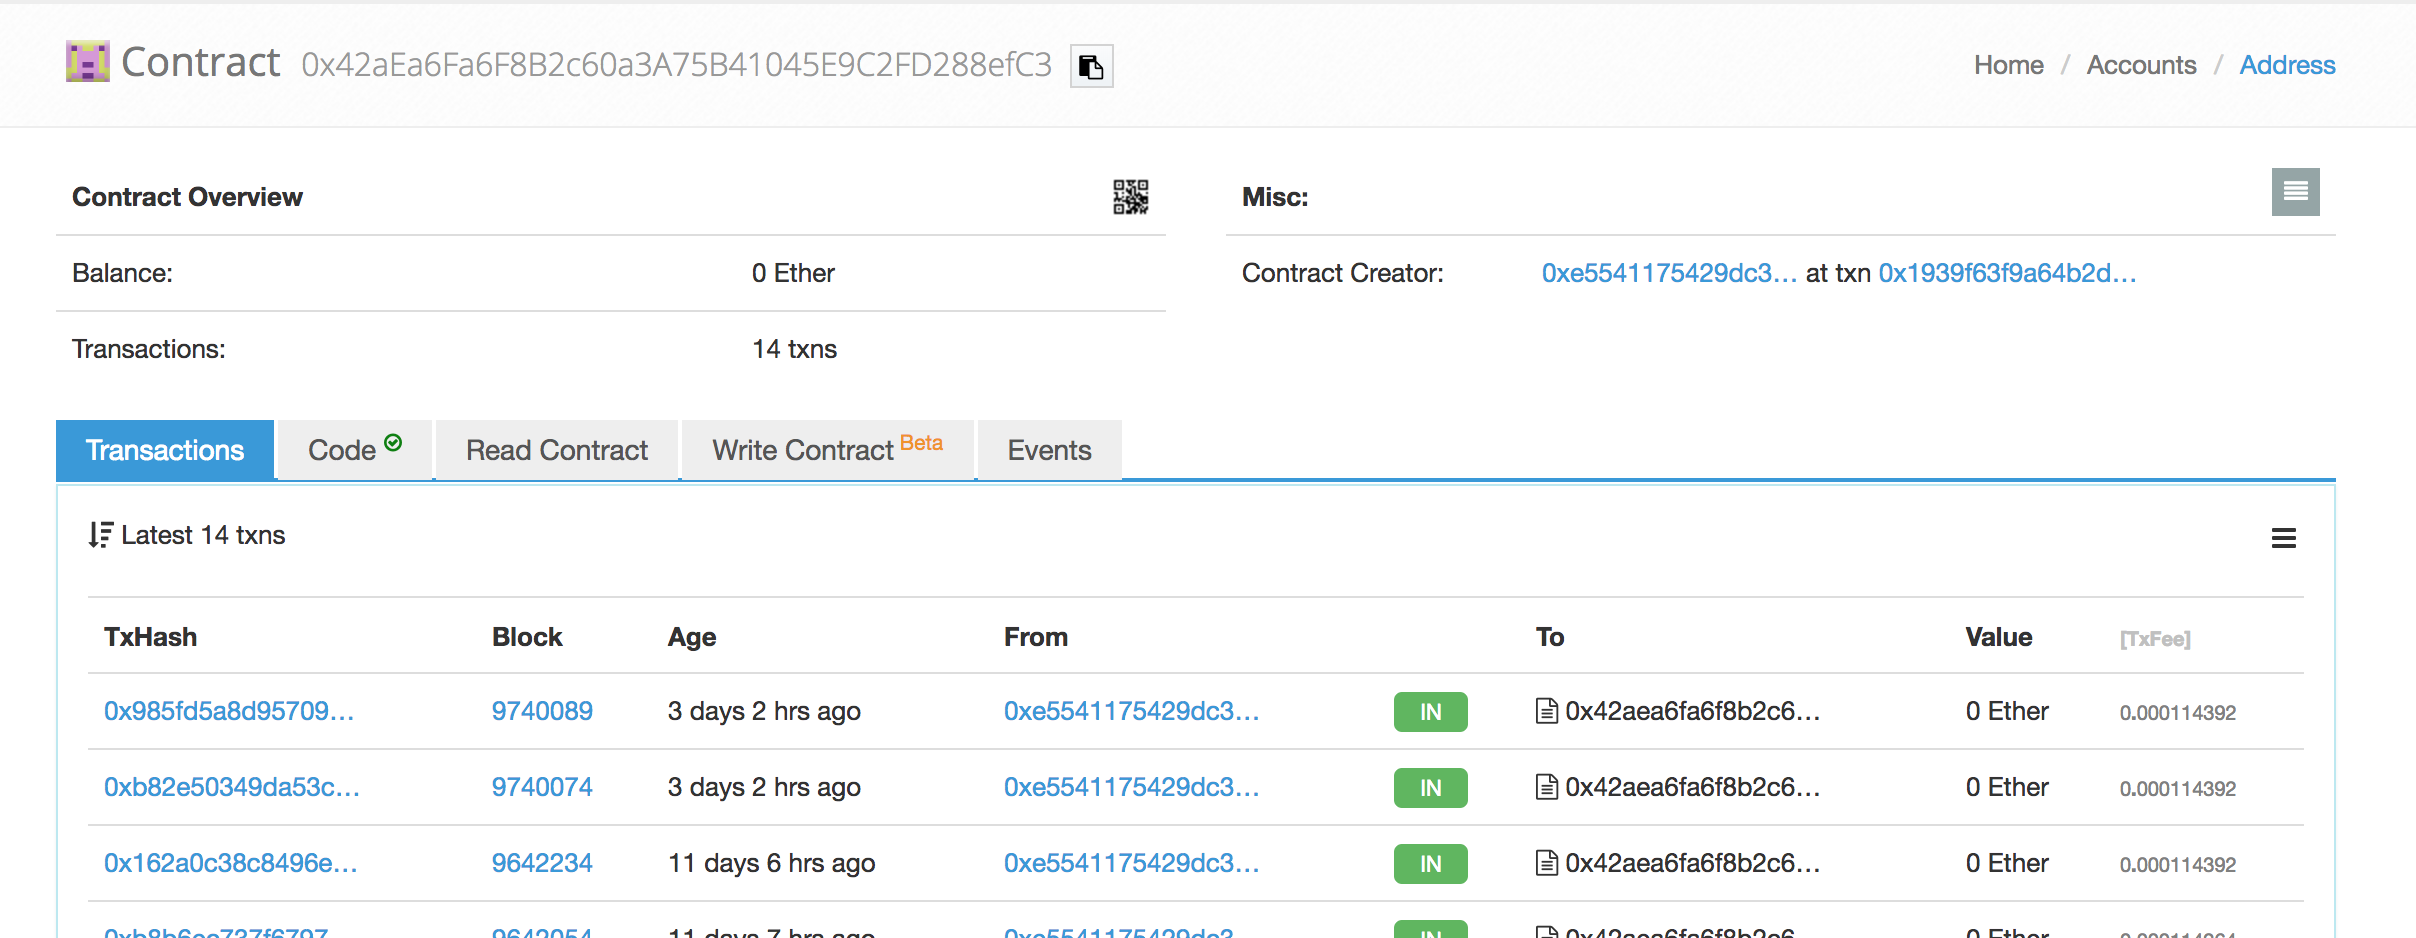
\includegraphics[height=6cm, width=13cm]{etherscan_transacciones.png}
  \centering
  \caption{Transacciones del contrato vistas desde Etherscan}
  \label{fig:etherscan-transacciones}
\end{figure}

Donde, como se puede ver, las últimas tres corresponden a las tres últimas que se vieron en la figura \ref{fig:listado-certificaciones}

En cuanto a los eventos disparados, se tienen los siguientes:

\begin{figure}[H]
  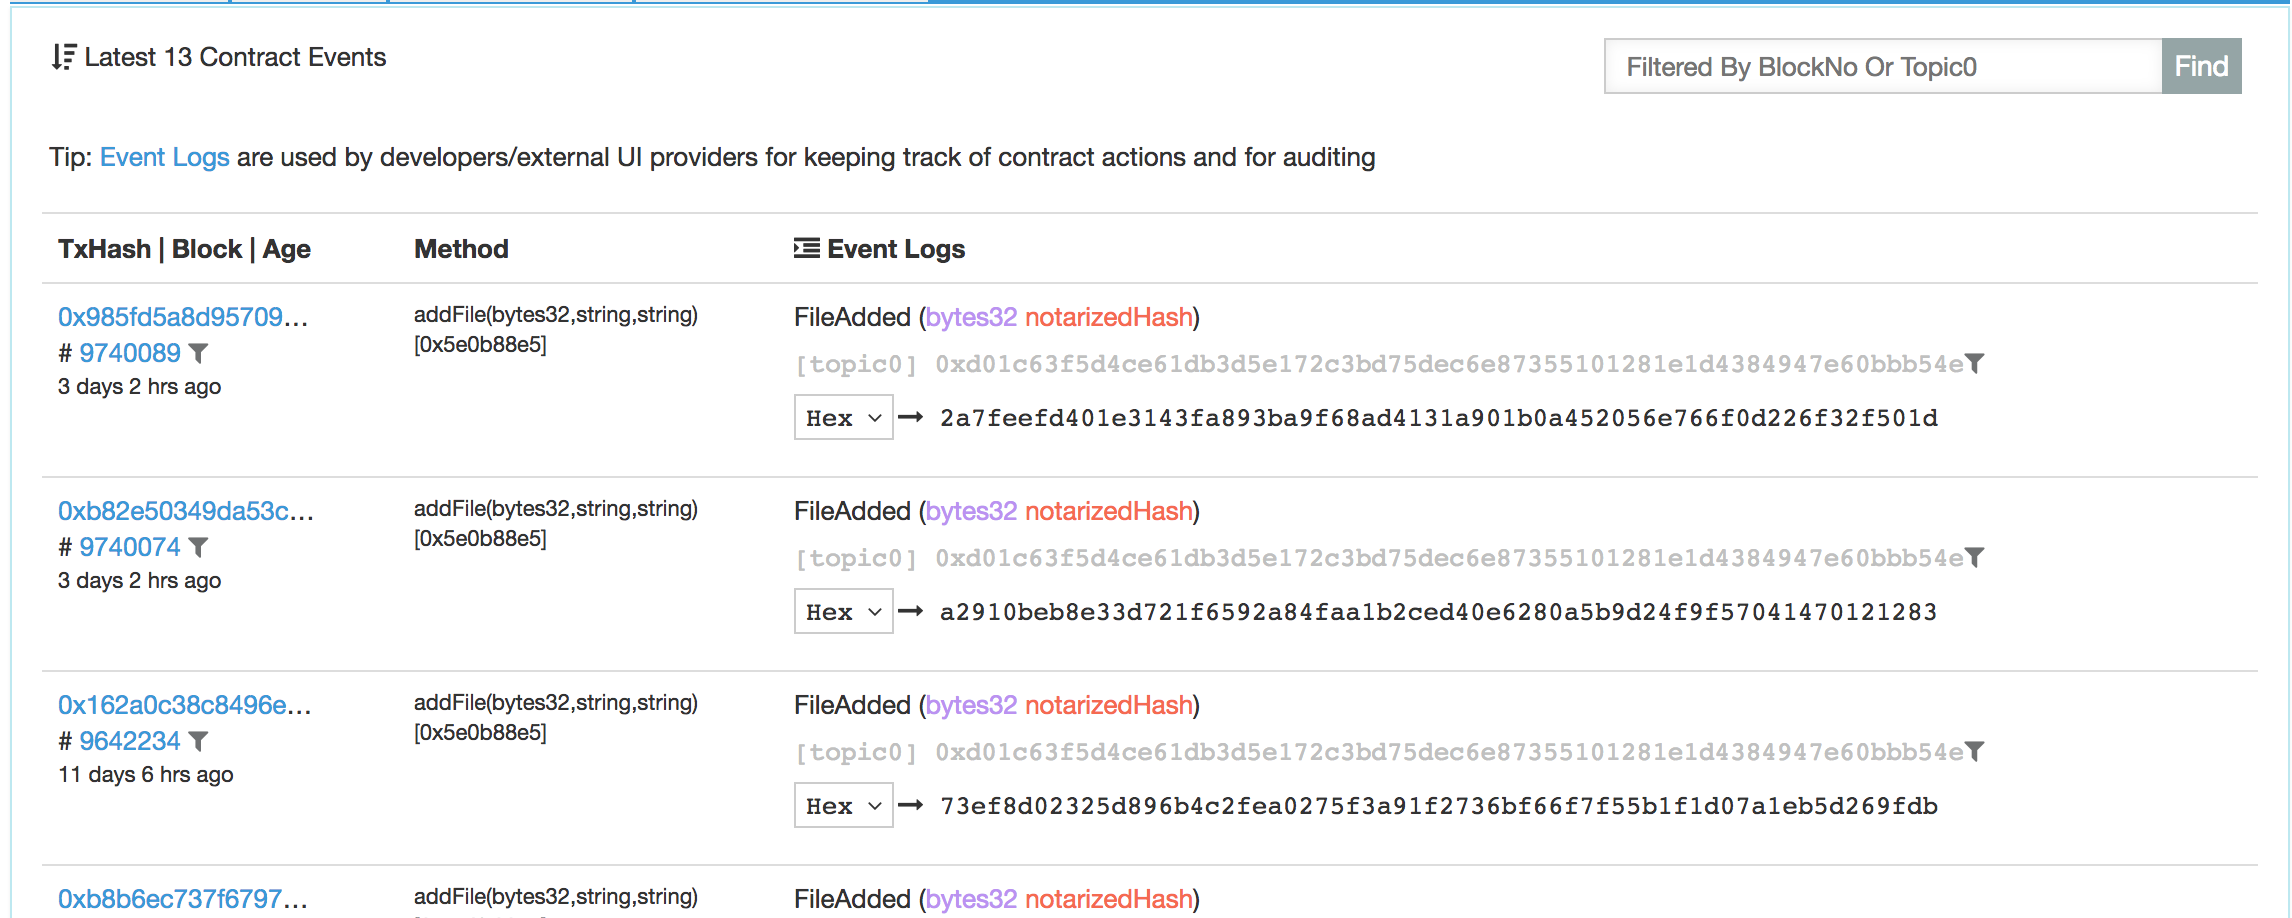
\includegraphics[height=6cm, width=13cm]{etherscan_eventos.png}
  \centering
  \caption{Eventos del contrato vistos desde Etherscan}
  \label{fig:etherscan-eventos}
\end{figure}

Que también se corresponden con las certificaciones vistas en la figura \ref{fig:listado-certificaciones}

En este punto debería quedar claro que la operación de listado confeccionada para la aplicación como parte del \textit{frontend}, es exactamente esto, una \textit{vista} que consume los datos directamente de la blockchain y los muestra de manera similar a como se ha visto en el apartado presente. Cualquiera con acceso a un explorador o un \textit{provider} conectados a la misma red deberán ver la misma información siempre, sin importar a cuál de los nodos elija conectarse.

\subsection{Recapitulación}
\label{recapitulacion_impl_solucion}

En esta sección se ha descrito en detalle las principales funcionalidades que aporta el prototipo del sistema que realiza certificaciones de archivos y usa la blockchain de Ethereum como \textit{backend} descentralizado. El objetivo buscado con esta arquitectura fue el de distribuir y replicar las transacciones con las huellas digitales -generadas desde una aplicación \textit{frontend}-  entre muchos nodos de manera implícita para que la confianza no recaiga en un único punto y, así, brindar mejoras sustanciales en cuanto a la seguridad y a la disponibilidad del servicio.
Se han discutido, en primer lugar, variantes dentro de la propia arquitectura en pos de lograr mayor control propio del mismo, pero sacrificando las bondades de la descentralización. Luego se han puesto en escena las especificaciones de las operaciones soportadas por el prototipo. Posteriormente, se brindaron detalles de la implementación de estas operaciones con gráficos demostrativos. Por último, se han podido explorar las transacciones generadas por la aplicación desde un explorador de la blockchain con el propósito de demostrar que los datos o las certificaciones generadas se pueden ver por fuera del sistema desarrollado y que accediendo a cualquier nodo de esta blockchain se van a visualizar exactamente los mismos datos.
